% T12 C/D, chapitre 10 : Fonctions exponentielle et logarithme. Source : le livre « Terminales scientifiques » (ExpoLog/Lesona, ExpoLog/Exo).
% Les exercices tirés d’autres ouvrages ne sont pas repris (décision du 2 novembre 2026).

\TCDLessonStyleOn
\chapter{Fonction exponentielle et logarithme}
\section{Fonction exponentielle}
      \begin{defi}
      \index{Fonction!exponentielle}
            La \emph{fonction exponentielle} est l'unique fonction $f$ d\'efinie sur $\mathbb{R}$ et v\'erifiant : 
                  \[   f' = f \qquad \text{ et } \qquad f(0) = 1   \,. \]
            On note la fonction par $\mathrm{exp}$.
      \end{defi}
      %
      \begin{prop}
            La fonction exponentielle peut en fait \^etre consid\'er\'e comme une fonction puissance.
            Il existe un nombre r\'eel $e$ ($\simeq 2,718\,281\,828\,459\,045$) 
            tel que $\exp{x} = e^{x}$ pour tout $x\in\mathbb{Q}$.
            
            Ainsi, dor\'enavant, on consid\`erera la fonction exponentielle comme 
            une g\'en\'eralisation d'une fonction puissance.
            On d\'enotera alors $\exp{x}$ par $\expo{x}$.
      \end{prop}
      %
      \begin{thm}
            Soient $a$ et $b$ deux nombres r\'eels.
            \begin{itemize}
                  \item $\expo{0} = 1$
                  \item $\expo{a+b} = \expo{a} \cdot \expo{b}$
                  \item $\expo{-a} = \frac{1}{\expo{a}}$
                  \item $\expo{a-b} = \frac{\expo{a}}{\expo{b}}$
                  \item $\forall n \in \mathbb{Q},\ \left(\expo{a}\right)^n = \expo{na}$.
            \end{itemize}
      \end{thm}
      %
      \begin{prop}
            La fonction $\exp$ est d\'efinie sur $\mathbb{R}$.
            De plus, $\expo{x} > 0$ pour tout $x\in\mathbb{R}$.
            Comme $\exp' x = \exp x > 0$, alors la fonction $\exp$ est strictement croissante sur $\mathbb{R}$.
            Il suit que, pour tout $(x,y)\in\mathbb{R}^2$ :
                  \[
                        x<y \Rightarrow \expo{x} < \expo{y}      \;.
                  \]
      \end{prop}
      %
      \begin{thm}[Limites usuelles sur la fonction $\exp$]
            \begin{align*}
                  \lim_{x\rightarrow-\infty} \expo{x} & = 0     & \lim_{x\rightarrow+\infty} \expo{x} & = +\infty \\
                  \lim_{x\rightarrow-\infty} x \expo{x} & = 0   & \lim_{x\rightarrow+\infty} \frac{\expo{x}}{x} & = +\infty \\
                \intertext{ou plus g\'en\'eralement, pour tout $n\in\mathbb{N}$}
                  \lim_{x\rightarrow-\infty} x^n \expo{x} & = 0 & \lim_{x\rightarrow+\infty} \frac{\expo{x}}{x^n} & = +\infty\;.
            \end{align*}
            On a aussi 
                  \[
                        \lim_{x\rightarrow 0} \frac{\expo{x}-1}{x} = 1      \;.
                  \]
      \end{thm}
      %
      \paragraph{Fonctions compos\'ees avec la fonction exponentielle}
            Il suit de la formule de d\'erivation d'une fonction compos\'ee que 
            $\left( \expo{u} \right)' = u' \expo{u}$.
            Ainsi, $u$ et $\expo{u}$ ont m\^eme sens de variations.
      \paragraph{\'Etude de la fonction $\exp$}~\\
      Posons $f(x) = \expo{x}$.
            \begin{description}
            \item[Domaine de d\'efinition :] La fonction $\exp$ est d\'efinie sur $\mathbb{R} = ]-\infty,+\infty[$.
            \item[Limites aux bornes :] $\lim_{x\rightarrow -\infty} \expo{x} = 0$ et 
                                        $\lim_{x\rightarrow +\infty} \expo{x} = +\infty$
            \item[D\'eriv\'ee :] Pour tout $x\in\mathbb{R}$, $f'(x) = \expo{x}$.
            \item[Tableau des variations :]~\\[-1\baselineskip]
                  \begin{table}[H]
                  \centering
                        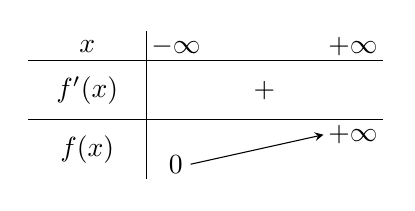
\begin{tikzpicture}[>=stealth,scale=.75]
                        \draw (-2,0) -- (4,0);
                        \draw (-2,-1) -- (4,-1);
                        \draw (0,.5) -- (0,-2);
                        \draw (-1,.25) node[] {$x$};
                        \draw (-1,-.5) node[] {$f'(x)$};
                        \draw (-1,-1.5) node[] {$f(x)$};
                        \draw (.5,.25) node[] {$-\infty$};
                        \draw (3.5,.25) node[] {$+\infty$};
                        \draw (2,-.5) node[] {$+$};
                        \draw (.5,-1.75) node[] {$0$};
                        \draw (3.5,-1.25) node[] {$+\infty$};
                        \draw[->] (.75,-1.75) -- (3,-1.25);
                        \end{tikzpicture}
                  \caption{Tableau des variations de la fonction exponentielle.}
                  \label{tab:variations expo}
                  \end{table}
            \item[Valeurs remarquables :] $f(0) = 1$ donc la courbe passe par le point de coordonn\'es $(0,1)$.
                                          De plus, la d\'eriv\'ee en ce point est \'egale \`a $1$,
                                          ce qui signifie que la pente de la tangente en ce point 
                                          est parall\`ele \`a la premi\`ere bissectrice.
                                          $f(1) = \expo{}$ donc la courbe passe par le point de coordonn\'es $(1,\expo{})$. 
            \item[Courbe repr\'esentative :]
                  Avant de tracer la courbe repr\'esentative de $f$, \'etudions d'abord ses branches infinies.
                  \begin{itemize}
                        \item Comme $\lim_{x\rightarrow-\infty} f(x) = 0$, 
                              alors la courbe admet la droite d'\'equation $y=0$ comme asymptote horizontale
                              au voisinage de $-\infty$.
                        \item Comme $\lim_{x\rightarrow+\infty} f(x) = +\infty$ et que
                              $\lim_{x\rightarrow+\infty} \frac{f(x)}{x} = +\infty$ alors
                              la courbe admet une branche parabolique suivant $y'Oy$.
                  \end{itemize}
            \begin{figure}[h!]
            \centering
                  \begin{tikzpicture}[line cap=round,line join=round,>=stealth,scale=.9]
                  \draw[->,color=black] (-4.2,0) -- (5.24,0);
                  \foreach \x in {-4,-3,-2,-1,1,2,3,4,5}
                  \draw[shift={(\x,0)},color=black] (0pt,2pt) -- (0pt,-2pt) node[below] {\footnotesize $\x$};
                  \draw[->,color=black] (0,-4.2) -- (0,5.3);
                  \foreach \y in {-4,-3,-2,-1,1,2,3,4,5}
                  \draw[shift={(0,\y)},color=black] (2pt,0pt) -- (-2pt,0pt) node[left] {\footnotesize $\y$};
                  \draw[color=black] (0pt,-10pt) node[right] {\footnotesize $0$};
                  \clip(-4,-4) rectangle (5.7,5.7);
                  \draw[dashed] (0,2.718281828) -- (1,2.718281828);
                  \draw[dashed] (1,0) -- (1,2.718281828);
                  \draw[color=loko1, smooth,samples=100,domain=0:1.6, thick] 
                                                                  plot(\x,{2.718281828^(\x)}) node[fill=white] {$y=\expo x$};
                  \draw[color=loko1, smooth,samples=100,domain=0:5, thick] plot({-\x},{1/(2.718281828^(\x))});
                  \draw[color=loko3, smooth,samples=100,domain=-4:4, thick] plot(\x,{(\x)+1}) node[fill=white] {$y=x+1$};
                  \filldraw[fill=loko1, draw=loko2] (0,1) circle (.2em);
                  \filldraw[fill=loko1, draw=loko2] (1,2.718281828) circle (.2em);
                  \end{tikzpicture}
            \caption{Courbe repr\'esentative de la fonction $\exp$.}
            \label{fig:courbe exp}
            \end{figure}
            \end{description}
            

\section{Fonction Logarithme}
      \subsection{Logarithme n\'ep\'erien}
      \begin{defi}
      \index{Fonction!Logarithme neperien@Logarithme n\'ep\'erien}
            On a vu que la fonction exponentielle est continue (elle est m\^eme d\'erivable)
            et strictement croissante sur $\mathbb{R}$.
            Elle d\'efinit donc une bijection de $\mathbb{R}$ vers $\mathbb{R}^*_+$.
            On définit la fonction logarithme népérien comme étant la fonction r\'eciproque de la fonction exponentielle.
            Ainsi, 
            $\ln : \mathbb{R}^*_+   \rightarrow   \mathbb{R}$ v\'erifie :
                  \[
                        \left\lbrace
                              \begin{array}{ll}
                                    \forall x\in\mathbb{R}      ,&  \ln(\expo{x}) = x \\
                                    \forall x\in\mathbb{R}^*_+  ,&  \expo{\ln x} = x  \;.
                              \end{array}
                        \right.
                  \]
      \end{defi}
      Ainsi, la courbe de la fonction $\exp$ et celle de la fonction $\ln$ sont 
      sym\'etriques par rapport \`a la premi\`ere bissectrice.
            \begin{figure}[h!]
            \centering
                  \begin{tikzpicture}[line cap=round,line join=round,>=stealth,scale=.9]
                  \draw[->,color=black] (-4.2,0) -- (5.24,0);
                  \foreach \x in {-4,-3,-2,-1,1,2,3,4,5}
                  \draw[shift={(\x,0)},color=black] (0pt,2pt) -- (0pt,-2pt) node[below] {\footnotesize $\x$};
                  \draw[->,color=black] (0,-4.2) -- (0,5.3);
                  \foreach \y in {-4,-3,-2,-1,1,2,3,4,5}
                  \draw[shift={(0,\y)},color=black] (2pt,0pt) -- (-2pt,0pt) node[left] {\footnotesize $\y$};
                  \draw[color=black] (0pt,-10pt) node[right] {\footnotesize $0$};
                  \clip(-4,-4) rectangle (5.7,5.7);
                  \draw[color=loko2, smooth,samples=100,domain=0.001:5, thick] 
                        plot(\x,{ln((\x))}) node[fill=white,sloped,above left] {$y=\ln x$};
                  \draw[color=loko1, smooth,samples=100,domain=0:1.6, thick] 
                                                                  plot(\x,{2.718281828^(\x)}) node[fill=white] {$y=\expo x$};
                  \draw[color=loko1, smooth,samples=100,domain=0:5, thick] plot({-\x},{1/(2.718281828^(\x))});
                  \draw[color=loko3, smooth,samples=100,domain=-4:5, thick] plot(\x,{(\x)}) node[fill=white] {$y=x$};
                  \end{tikzpicture}
            \caption{Courbe des fonctions $\exp$ et $\ln$.}
            \label{fig:exp et ln}
            \end{figure}
      %
      \begin{rmk}[Valeurs remarquables]~\\[-1\baselineskip]
            \begin{itemize}
                  \item $\ln 1 = 0$ car $\expo{0} = 1$
                  \item $\ln \expo{} = 1$ car $\expo{1} = \expo{}$.
            \end{itemize}
            Comme la fonction exponentielle est continue et strictement croissante de $\mathbb{R}$ sur $]0,+\infty[$, 
            la fonction Logarithme n\'ep\'erienne est continue et strictement croissante $]0,+\infty[$ sur $\mathbb{R}$.
      \end{rmk}
      %
      \begin{prop}[Propri\'et\'es alg\'ebriques]
            Soient $a$ et $b$ deux nombres r\'eels positifs et $n$ un entier relatif.
            On a alors :\\
            \begin{align*}
                        \ln (a\cdot b) & = \ln a + \ln b                                                &       
                        \ln (a^n) & = n \cdot \ln a                                                     \\
                        \ln \frac{1}{a} & = - \ln a                                                     & 
                        \ln \frac{a}{b} & = \ln a - \ln b                                               \\
                        \ln a < \ln b & \iff a < b                                                      & 
                        \ln a = \ln b & \iff a = b                                                      \\
                        \forall \lambda \in \mathbb{R},\ \ln x = \lambda & \iff x = \expo{\lambda}      & 
                        \forall \lambda \in \mathbb{R}^*_+,\ \expo{x} = \lambda & \iff x = \ln{\lambda} \\
                        \forall \lambda \in \mathbb{R},\ \ln x < \lambda & \iff x < \expo{\lambda}      & 
                        \forall \lambda \in \mathbb{R}^*_+,\ \expo{x} < \lambda & \iff x < \ln{\lambda} \\
            \end{align*}
      \end{prop}
      %
      \begin{thm}[D\'eriv\'ee de la fonction $\ln$]
            La fonction logarithme n\'ep\'erien est d\'erivable sur $]0,+\infty[$ avec
                  \begin{equation*}
                        \left( \ln x \right)' = \frac{1}{x}      \;.
                  \end{equation*}
            \begin{proof}
                  Posons $f(x) = \expo{x}$. On sait alors que $f^{-1} (x) = \ln x$.
                  En utilisant la formule de d\'erivation de la fonction r\'eciproque, on a :
                        \begin{align*}
                              \left(f^{-1}\right)' (x)  & = \frac{1}{f' \left( f^{-1} (x) \right) }      \\
                              \left(\ln (x) \right)'    & = \frac{1}{\expo{\ln x}}                       \\
                              \left(\ln (x) \right)'    & = \frac{1}{x}                                  \,.
                        \end{align*}
            \end{proof}
      \end{thm}
      %
      \begin{thm}[Limites usuelles]~\\
                  \begin{align*}
                        \lim_{x\rightarrow 0^+} \ln x                & = -\infty            &
                        \lim_{x\rightarrow 0^+} x\cdot\ln x          & = 0                  \\
                        \lim_{x\rightarrow +\infty} \ln x            & = +\infty            &
                        \lim_{x\rightarrow +\infty} \frac{\ln x}{x}  & = 0                  
                  \end{align*}
                  \[
                        \lim_{x\rightarrow 0} \frac{\ln (1 + x)}{x} = 1      \;.
                  \]
      \end{thm}
      %
      \paragraph{Fonctions compos\'ees avec la fonction logarithme n\'ep\'erien}
            Soit $u$ une fonction d\'erivable sur un intervalle $I$ tel que $u(x)>0$ pour tout $x\in I$.
            Il suit de la formule de d\'erivation d'une fonction compos\'ee que 
            $\left( \ln {u} \right)' = \frac{u'}{u}$.
            Ainsi, $u$ et $\ln{u}$ ont m\^eme sens de variations.
      %
            
      %
      \subsection{Logarithme de base quelconque}
            \begin{defi}[Logarithme d\'ecimal]
                  On d\'efinit la fonction logarithme d\'ecimal par :
                        \begin{equation*}
                              \begin{array}{rcl}
                                    \log :\ ]0,+\infty[ & \rightarrow & \mathbb{R}      \\
                                                     x & \mapsto     & \frac{\ln x}{\ln 10}
                              \end{array}
                        \end{equation*}
            \end{defi}
            %
            \begin{prop}
                  Si la fonction $\ln$ est la r\'eciproque de la fonction $x\mapsto \expo{x}$,
                  la fonction $\log$ peut \^etre consid\'er\'ee comme \'etant la r\'eciproque de la fonction $x\mapsto 10^x$.
                  
                  Ainsi, si $n$ est un nombre entier naturel, l'\'ecriture d\'ecimale de $n$ comporte 
                  $\entiere{\log (n)}+1$ chiffres.
                        \begin{ex}
                              Le plus grand nombre premier connu \`a ce jour (mai 2018)%
                                    \footnote{%
                                    D\'ecouvert en d\'ecembre 2017 par le GIMPS en d\'ecembre 2017.
                                                }
                              est $2^{77\, 232\, 917} - 1$.
                              Puisqu'il s'agit d'un nombre premier, 
                              il comporte le m\^eme nombre de chiffre que le nombre $2^{77\, 232\, 917}$.
                              Pour calculer le nombre de chiffres qu'il comporte, on effectue :
                                    \[
                                           \log (2^{77\, 232\, 917})
                                    =      \frac{\ln (2^{77\, 232\, 917})}{\ln 10} 
                                    =      \frac{77\, 232\, 917 \cdot \ln 2}{\ln 10}
                                    \simeq 23\,249\,424,66962662
                                    .
                                    \]
                              Ainsi, ce nombre comporte $23\,249\,425$ chiffres.
                        \end{ex}
            \end{prop}
            \begin{defi}[Logarithme de base $a$]
                  Soit $a$ un nombre r\'eel strictement positif.
                  On d\'efinit la fonction logarithme de base $a$ par :
                        \begin{equation*}
                              \begin{array}{rcl}
                                    \log_a :\ ]0,+\infty[ & \rightarrow & \mathbb{R}                        \\
                                                        x & \mapsto     & \frac{\ln x}{\ln a}               \;.
                              \end{array}
                        \end{equation*}
            \end{defi}
      %
      




\TCDLessonStyleOff
\clearpage
\providecommand{\ivec}{\vec{\imath}}
\providecommand{\jvec}{\vec{\jmath}}
\providecommand{\Oij}{$(O,\ivec,\jvec)$ }
%%%%%%%%%%%%%%%%%%%%%%%%%%%%%%%%%%%%%%%%%%%%%%%%%%%%%%%%%%%%%%%%%%%%%%%%%%%%%%%%%%%
%%%%%%%%%%%%%%%%%%%%%%%%%%%%%%%%%%%%%%%%%%%%%%%%%%%%%%%%%%%%%%%%%%%%%%%%%%%%%%%%%%%
\section{Exercices}
%%%%%%%%%%%%%%%%%%%%%%%%%%%%%%%%%%%%%%%%%%%%%%%%%%%%%%%%%%%%%%%%%%%%%%%%%%%%%%%%%%%
\begin{exo}
\begin{description}
\item[A.] On consid\`ere la fonction $\varphi$ d\'efinie sur $\mathbb{R}$ par $\varphi(x) = \expo{x} + x + 1$.
      \begin{enumerate}
      \item Dresser le tableau des variations complet de $\varphi$.
      \item Montrer que l'\'equation $\varphi (x) = 0$ admet une unique solution $\alpha$ et que 
            ${\alpha \in \ ] -1,28 \ ; \ -1,27 [}$.
      \item En d\'eduire le signe de $\varphi (x)$ sur $\mathbb{R}$.
      \end{enumerate}
\item[B.] Soit $f$ la fonction d\'efinie sur $\mathbb{R}$ par $f(x) = \frac{x \expo{x}}{\expo{x} + 1}$ et notons par 
      $(\mathcal{C})$ sa courbe repr\'esentative dans un rep\`ere orthonorm\'e $(O , \ivec , \jvec )$ d'unit\'e $4 \text{cm}$.
      \begin{enumerate}
      \item Etudier les variations de $f$.
      \item Montrer que $f(\alpha) = \alpha + 1$.
      \item Calculer les limites de $f$ aux bornes de $\mathbb{R}$ et montrer que la droite $(\mathcal{D})$ d'\'equation 
            $y = x$ est asymptote \`a $(\mathcal{C})$ et \'etudier la position de $(\mathcal{C})$ par rapport \`a $(\mathcal{D})$.
      \item Tracer $(\mathcal{C})$ et $(\mathcal{D})$ dans le m\^eme rep\`ere.
      \end{enumerate}
\end{description}
\end{exo}
%%%%%%%%%%%%%%%%%%%%%%%%%%%%%%%%%%%%%%%%%%%%%%%%%%%%%%%%%%%%%%%%%%%%%%%%%%%%%%%%%%%
\begin{exo} ~ \newline
Soit la fonction num\'erique $f$ d\'efinie sur l'intervalle $]-1 \; ; \; +\infty[$ par :
\begin{displaymath}
f(x) = 
\left\lbrace
\begin{tabular}{lll}
$ - x + 2 \ln (x + 1) $ & si & $ x \in \; ] -1 \; ; \; 0[ $ \\
$ x - 1 + \expo{-x} $ & si & $ x \in [0 \; ; \; + \infty[ $.
\end{tabular}
\right.
\end{displaymath}
On note par $(\mathscr{C})$ sa courbe repr\'esentative dans un rep\`ere orthonorm\'e \Oij d'unit\'e 2 cm.
\begin{enumerate}
\item Montrer que $f$ est continue en $0$.
\item Montrer que $\lim_{x \rightarrow 0^-} \frac{f(x) - f(0)}{x - 0} = 1$ et 
      $\lim_{x \rightarrow 0^+} \frac{f(x) - f(0)}{x - 0} = 0$.
      Que peut-on en conclure sur $f$\,?
\item \begin{enumerate}
      \item Calculer $\lim_{x \rightarrow -1^+} f(x)$ et $\lim_{x \rightarrow +\infty} f(x)$.
      \item Etudier le signe de $f'(x)$ sur les intervalles $]-1 \; ; \; 0[$ et $] 0 \; ; \; +\infty[$.
      \item Dresser le tableau des variations de $f$.
      \end{enumerate}
\item Montrer que la droite $(\mathcal{D})$ d'\'equation $y = x- 1$ est asymptote \`a $(\mathscr{C})$ au voisinage de $+\infty$.
\item Tracer $(\mathscr{C})$ et $(\mathcal{D})$ dans le m\^eme rep\`ere \Oij en pr\'ecisant les demi-tangentes \`a l'origine.
\item Soit $g$ la restriction de $f$ \`a l'intervalle $I = [ 0 \; ; \; +\infty[$.
      \begin{enumerate}
      \item Montrer que $g$ admet une r\'eciproque $g^{-1}$ dont on d\'eterminera l'ensemble de d\'efinition.
      \item Repr\'esenter $g^{-1}$ dans le m\^eme rep\`ere que $(\mathscr{C})$.
      \end{enumerate}
\end{enumerate}

\end{exo}
%%%%%%%%%%%%%%%%%%%%%%%%%%%%%%%%%%%%%%%%%%%%%%%%%%%%%%%%%%%%%%%%%%%%%%%%%%%%%%%%%%%
\begin{exo} ~ \newline
Soit $f$ la fonction d\'efinie sur $\mathbb{R}$ par 
\begin{displaymath}
f(x) = 
\left\lbrace
\begin{matrix}
x - 2 - \ln ( e - x) & \text{ si } & x < 0     \\
\expo{x} \; (x^2 - 3)   & \text{ si } & x \geq 0  \; .
\end{matrix}
\right.
\end{displaymath}
On note $(\mathscr{C})$ sa courbe repr\'esentative dans un rep\`ere orthonorm\'e \Oij d'unit\'e 1~cm.
\begin{enumerate}
\item \begin{enumerate}
      \item Etudier la continuit\'e de $f$ en $0$.
      \item Montrer que $f$ est d\'erivable \`a gauche en $0$ et que $f'_g (0) = 1 + \frac{1}{e}$.
      \item Montrer que $f$ est d\'erivable \`a droite en $0$ et calculer $f'_d (0)$. Que peut-on en conclure?
      \end{enumerate}
\item \begin{enumerate}
      \item Etudier les variations de $f$.
      \item D\'eterminer les branches infinies de $(\mathscr{C})$.
      \item Montrer que $(\mathscr{C})$ coupe la premiere bissectrice au point d'abscisse $\alpha \in \; \left] \sqrt{3} \; ; \; 2 \right[$. 
            (On ne demande pas de calculer la valeur de $\alpha$)
      \end{enumerate}
\item Tracer la courbe $(\mathscr{C})$ en pr\'ecisant les demi-tangentes au point d'abscisse $0$.
\end{enumerate}
\end{exo}
%%%%%%%%%%%%%%%%%%%%%%%%%%%%%%%%%%%%%%%%%%%%%%%%%%%%%%%%%%%%%%%%%%%%%%%%%%%%%%%%%%%
% Manomboka eto ny log
%%%%%%%%%%%%%%%%%%%%%%%%%%%%%%%%%%%%%%%%%%%%%%%%%%%%%%%%%%%%%%%%%%%%%%%%%%%%%%%%%%%
\begin{exo} ~ \newline
On consid\`ere la fonction $f$ d\'efinie sur $I = ]0 \; ; \; +\infty[$ par $f(x) = x + \frac{2 \; \ln (x) }{x}$.
On d\'esigne par $(\mathscr{C})$ sa courbe repr\'esentative dans un rep\`ere orthonorm\'e \Oij d'unit\'e 1cm.
\begin{enumerate}
\item Soit $g$ la fonction d\'efinie par $g(x) = x^2 + 2 - 2 \; \ln (x)$.
      Etudier les variations de $g$ et en d\'eduire le signe de $g(x)$.
\item \begin{enumerate}
      \item Calculer les limites de $f$ aux bornes de son domaine de d\'efinition.
      \item Dresser le tableau des variations de $f$.
      \item Montrer que la droite $(\mathcal{D})$ d'\'equation $y = x$ est asymptote \`a $(\mathscr{C})$ et 
            \'etudier la position de $(\mathscr{C})$ par rapport \`a $(\mathcal{D})$.
      \item On d\'esigne par $A$ le point de $(\mathscr{C})$ o\`u la tangente $(T)$ est parall\`ele \`a $(\mathcal{D})$.
            D\'eterminer les coordonn\'ees du point $A$.
      \item Tracer $(\mathscr{C})$, $(\mathcal{D})$ et $(T)$ dans le rep\`ere \Oij.
      \end{enumerate}
\item Montrer que l'\'equation $f(x) = 0$ admet une solution unique $\alpha$ et 
      montrer que $\alpha \in \left] \frac{1}{2} \; ; \; 1 \right[$.
\end{enumerate}
\end{exo}
%%%%%%%%%%%%%%%%%%%%%%%%%%%%%%%%%%%%%%%%%%%%%%%%%%%%%%%%%%%%%%%%%%%%%%%%%%%%%%%%%%%
\begin{exo} 
\begin{description}
\item[A.] On consid\`ere la fonction $g$ d\'efinie sur $]0 \; ; \; +\infty[$ par 
      $g(x) = \ln \left( \frac{x+1}{x} \right) - \frac{1}{x+1}$.
      \begin{enumerate}
      \item D\'eterminer les limites de $g$ aux bornes de son domaine de d\'efinition.
      \item Dresser le tableau de variation de $g$.
            En d\'eduire le signe de $g(x)$ pour $x > 0$.
      \end{enumerate}
\item[B.] On consid\`ere la fonction $f$ d\'efinie sur $]0 \; ; \; +\infty[$ par 
      $f(x) = x \; \ln \left( \frac{x+1}{x} \right)$.
      \begin{enumerate}
      \item Calculer les limites de $f$ aux bornes de son domaine de d\'efinition.
      \item Dresser le tableau de variation de la fonction $f$.
      \item Tracer la courbe $(\mathscr{C})$ repr\'esentative de $f$.
      \end{enumerate}
\end{description}
\end{exo}
%%%%%%%%%%%%%%%%%%%%%%%%%%%%%%%%%%%%%%%%%%%%%%%%%%%%%%%%%%%%%%%%%%%%%%%%%%%%%%%%%%%
\begin{exo} ~ \newline
Soit $f$ la fonction d\'efinie par $f(x) = - \frac{x}{2} + \ln \left| \frac{x-1}{x} \right| $.
\begin{enumerate}
\item D\'eterminer l'ensemble de d\'efinition $\mathcal{D}f$ de $f$.
\item Etudier les variations de $f$.
\item On d\'esigne par $(\mathscr{C})$ la courbe repr\'esentative de $f$ dans un rep\`ere orthonorm\'e \Oij d'unit\'e 2~cm.
      Montrer que la droite $(\mathcal{D})$ d'\'equation $y = -\frac{x}{2}$ est asymptote \`a $(\mathscr{C})$ \hspace{-4pt}.
      Pr\'eciser la position de $(\mathscr{C})$ par rapport \`a $(\mathcal{D})$.
\item Montrer que le point $I \left( \frac{1}{2} ; -\frac{1}{4} \right)$ est centre de sym\'etrie de $(\mathscr{C})$ \hspace{-4pt}.
\item Donner une \'equation de la tangente \`a $(\mathscr{C})$ au point $I$.
\item Construire $(\mathscr{C})$ \hspace{-4pt}.
\item Montrer que l'\'equation $f(x)=0$ admet une solution r\'eelle unique $\alpha$ et que $\frac{2}{5} < \alpha < \frac{9}{20}$.
\end{enumerate}
\end{exo}
%%%%%%%%%%%%%%%%%%%%%%%%%%%%%%%%%%%%%%%%%%%%%%%%%%%%%%%%%%%%%%%%%%%%%%%%%%%%%%%%%%%
\begin{exo} ~ \newline
Soit la fonction $f$ d\'efinie par $f(x) = \frac{x^2 - 1}{4} - 2 \; \ln (x)$.
\begin{enumerate}
\item \begin{enumerate}
      \item Montrer que l'\'equation $f(x) = 0$ poss\`ede deux solutions et deux seulement 
            dont l'une \'egale \`a $1$ et l'autre $\alpha$ appartient \`a l'intervalle $[3 \; ; \; 4]$. 
            (On ne demande pas de calculer $\alpha$)
      \item Montrer que $\alpha = \sqrt{1 + 8 \; \ln \alpha}$.
      \end{enumerate}
\item Soit la fonction $h$ d\'efinie par $h(x) = \sqrt{1 + 8 \; \ln (x)}$ sur $[3 \; ; \; +\infty[$.
      Montrer que $h(x) \geq 3$ et que $0 \leq h'(x) \leq \frac{4}{9}$.
\item Soit la suite $(U_n)$ d\'efinie par $U_0 = 3$ et $U_{n+1} = h(U_n)$.
      Montrer par r\'ecurrence que, pour tout $n \in \mathbb{N}$, $U_n \geq 3$.
\item \begin{enumerate}
      \item Montrer que pour tout $n \in \mathbb{N}$ : 
            $\left| U_{n+1} - \alpha \right| \leq \frac{4}{9} \; \left| U_n - \alpha \right| $.
      \item Montrer que pour tout $n \in \mathbb{N}$ : 
            $\left| U_n - \alpha \right| \leq \left( \frac{4}{9} \right)^n $.
            En d\'eduire que la suite $(U_n)$ est convergente.
      \item Trouver un entier $n_0$ tel que $\left| U_{n_0} - \alpha \right| < 10^{-2}$.
            En d\'eduire une approximation de $\alpha$ \`a $10^{-2}$ pr\`es.
      \end{enumerate}
\end{enumerate}
\end{exo}
%%%%%%%%%%%%%%%%%%%%%%%%%%%%%%%%%%%%%%%%%%%%%%%%%%%%%%%%%%%%%%%%%%%%%%%%%%%%%%%%%%%
\begin{exo}
Soit $k$ un r\'eel strictement positif. On d\'efinit alors la fonction $g_k$ par : $$ g_k (x) = e^{- k x^2} \; .$$
\begin{enumerate}
\item \'Etudier la parit\'e de la fonction $g_k$.
\item D\'emontrer que $g_k$ est d\'erivable et donner sa d\'eriv\'ee $g'_k$.
\item \'Etudier le signe de $g'_k (x)$ puis dresser le tableau de variation de $g_k$.
\item Exprimer $g''_k (x)$ en fonction de $x$ et r\'esoudre l'\'equation $g''_k (x) = 0$.
\item Tracer la courbe de $g_{\frac{1}{2}}$ , $g_1$ et $g_2 $.
\item D\'emontrer que, sur $\mathbb{R}$ : 
      $$ h \leq k \iff g_h \geq g_k  \; .$$
\item Dans cette question, $k = \frac{1}{2}$.
      Soit $\alpha$ la solution positive de l'\'equation $g''_k (x) = 0$.
      D\'eterminer une \'equation de la tangente $(T )$ \`a la courbe repr\'esentative de $g_k$ au point d'abscisse $\alpha$. 
      Tracer $(T )$.
\end{enumerate}
\end{exo}
%%%%%%%%%%%%%%%%%%%%%%%%%%%%%%%%%%%%%%%%%%%%%%%%%%%%%%%%%%%%%%%%%%%%%%%%%%%%%%%%%%%
\begin{exo}
~ \newline
%%%%%%%%%%%%%%%%%%%%%%%%%%%%%%%%%
\textbf{Partie A} \newline
\begin{enumerate}
\item D\'emontrer que pour tout r\'eel positif ou nul $x$ : $ \displaystyle{ e^{x} - \frac{x^2}{2} \geq 1 }$.
\item En d\'eduire $\lim_{x \rightarrow + \infty} \frac{e^x}{x}$.
\end{enumerate}
%%%%%%%%%%%%%%%%%%%%%%%%%%%%%%%%%
\textbf{Partie B} \newline
On consid\`ere la fonction $g$ d\'efinie sur $\mathbb{R}$ par : $ \displaystyle{ g(x) = 2e^x - x - 2 }$.
\begin{enumerate}
\item D\'eterminer la limite de g en $- \infty$ puis en $+ \infty$.
\item \'Etudier le sens de variation de $g$ puis dresser son tableau de variations.
\item \begin{enumerate}
      \item Montrer que $x = 0$ est solution de l'\'equation $g(x) = 0$.
      \item Montrer que l'\'equation $g(x) = 0$ admet une deuxi\`eme solution $\alpha$ sur l'intervalle $]-1, 6 ; -1, 5[$.
      \end{enumerate}
\end{enumerate}
%%%%%%%%%%%%%%%%%%%%%%%%%%%%%%%%%
\textbf{Partie C} \newline
On consid\`ere la fonction $f$ d\'efinie sur $\mathbb{R}$ par : $ \displaystyle{  f(x) = e^{2x} - (x+1) e^x }$.
\begin{enumerate}
\item D\'eterminer la limite de $f$ en $- \infty$ puis en $+ \infty$.
\item Calculer $f'(x)$. D\'eduire de la {Partie B} le signe de $f'(x)$ sur $\mathbb{R}$.
\item Montrer que : 
      $ \displaystyle{ 
      f(\alpha) = - \frac{\alpha^2 + 2 \alpha}{4}
      }
      $
      o\`u $\alpha$ est d\'efinie dans la partie pr\'ec\'edente.
      En d\'eduire un encadrement de $f (\alpha)$.
\item Dresser un tableau de variations de $f$ .
\item Tracer la courbe $(\mathscr{C})$, repr\'esentative de $f$, dans le plan rapport\'e \`a un rep\`ere orthonormal (unit\'e graphique : 2cm).
\end{enumerate}
%%%%%%%%%%%%%%%%%%%%%%%%%%%%%%%%%
\end{exo}
%%%%%%%%%%%%%%%%%%%%%%%%%%%%%%%%%%%%%%%%%%%%%%%%%%%%%%%%%%%%%%%%%%%%%%%%%%%%%%%%%%%
\begin{exo}
Soit $f$ la fonction d\'efinie sur $\mathbb{R}$ par 
$\displaystyle{f(x) = \frac{ 2 \expo{x} }{ \expo{x} + \expo{-x} } }$.
On note par $(\mathscr{C})$ sa courbe repr\'esentative 
dans un rep\`ere orthonorm\'e $(O,\vec{\imath},\vec{\jmath})$ d'unit\'e 2cm.
\begin{enumerate}
      \item Dresser le tableau de variation de $f$.
            En d\'eduire que $f$ admet une fonction r\'eciproque $f^{-1}$ dont on d\'eterminera le domaine de d\'efinition.
            On note par $(\mathscr{C}')$ la courbe repr\'esentative de $f^{-1}$.
      \item Montrer que $f$ admet un point d'inflexion $I$ dont on d\'eterminera les coordonn\'ees.
            Montrer que $I$ est un centre de sym\'etrie de la courbe $(\mathscr{C})$.
      \item Donner une \'equation cart\'esienne de la droite $(T)$, tangente \`a $(\mathscr{C})$ au point $I$.
            Tracer $(\mathscr{C})$, $(\mathscr{C}')$ ansi que leurs asymptotes dans le m\^eme rep\`ere.
\end{enumerate}
\end{exo}
%%%%%%%%%%%%%%%%%%%%%%%%%%%%%%%%%%%%%%%%%%%%%%%%%%%%%%%%%%%%%%%%%%%%%%%%%%%%%%%%%%%
\begin{exo}
\textbf{Partie A}
Soit $g$ la fonction d\'efinie par : $g(x) = (\ln x)^3 + \ln x - 2$.
\begin{enumerate}
\item Donner le domaine de d\'efinition de $g$.
\item Donner la fonction d\'eriv\'ee de $g$ et \'etudier son signe.
      En d\'eduire la variation de la fonction $g$
\item Calculer $g(e)$ et en d\'eduire le signe de $g(x)$ en fonction de $x$.
\end{enumerate}
\textbf{Partie B}
Soit $f$ la fonction d\'efinie par : $ f(x) = \frac{(\ln x)^3 - \ln x + 1}{(\ln x)^2}$ .
\begin{enumerate}
\item 
      \begin{enumerate}
      \item D\'eterminer l'ensemble de d\'efinition $\mathcal{D}f$ de $f$. 
      \item Calculer les limites de $f$ aux bornes de $\mathcal{D}f$.
      \end{enumerate}
\item 
      \begin{enumerate}
      \item Montrer que $f$ est d\'erivable sur $\mathcal{D}f$ et que pour tout $x$ de $\mathcal{D}f$ : 
            $f'(x) = \frac{g(x) \; \ln x}{x \; (\ln x)^4}$.
      \item Etudier les variations de $f$.
      \end{enumerate}
\item Dans le plan muni d'un rep\`ere orthonorm\'e,
      on consid\`ere la courbe $(\mathscr{C})$ repr\'esentative de $f$ et la courbe $(\Gamma)$ d\'equation $y = \ln x$.
      \begin{enumerate}
      \item Etudier la position relative de $(\mathscr{C})$ et de $(\Gamma)$.
      \item Tracer $(\mathscr{C})$ et $(\Gamma)$ sur le m\^eme graphique.
      \end{enumerate}
\end{enumerate}
\end{exo}
%%%%%%%%%%%%%%%%%%%%%%%%%%%%%%%%%%%%%%%%%%%%%%%%%%%%%%%%%%%%%%%%%%%%%%%%%%%%%%%%%%%
\begin{exo}
      On consid\`ere la fonction $f$ de la variable r\'eelle $x$ d\'efinie par $f(x) = 2 x + \ln \left| \frac{x + 1}{x} \right|$.
      On d\'esigne par $(\mathcal{C})$ la courbe repr\'esentative de $f$ dans un rep\`ere orthonorm\'e $(O,\vec{\imath}, \vec{\jmath})$ d'unit\'e 1~cm.
      \begin{enumerate}
      \item Donner l'ensemble de d\'efinition de $f$ et calculer les limites de $f$ aux bornes de son domaine de d\'efinition.
      \item Etudier les variations de la fonction $f$.
      \item 
            \begin{enumerate}
            \item D\'emontrer que la droite $(D)$ d'\'equation $y = 2x$ est asymptote \`a $(\mathcal{C})$.
            \item Etudier la position de $(\mathcal{C})$ par rapport \`a $(D)$.
            \item Tracer $(\mathcal{C})$.
            \end{enumerate}
      \item Soit $g$ la restriction de $f$ \`a $]-1 ; 0[$. Montrer que l'\'equation $g(x) = 0$ admet une racine $\alpha \in ]-\frac{1}{2} ; \frac{1}{2}[$ et une seule.
      \item 
           \begin{enumerate}
           \item On pose $k(x) = \ln (x + a)$ avec $a \in \mathbb{R}$.
                 D\'eterminer une primitive de $k$ dans l'intervalle $]-a ; + \infty[$.
           \item En d\'eduire l'aire du domaine-plan limit\'e par $(\mathcal{C})$, $(D)$ et les droites d'\'equation $x = 1$ et $x = 2$.
           \end{enumerate}
      \end{enumerate}
\end{exo}
%%%%%%%%%%%%%%%%%%%%%%%%%%%%%%%%%%%%%%%%%%%%%%%%%%%%%%%%%%%%%%%%%%%%%%%%%%%%%%%%%%%
\begin{exo}
      Soit $f$ la fonction d\'efinie par $f(x) = 2 x + \frac{e^x}{e^x - 1}$ et notons par $(\mathcal{C})$ sa courbe repr\'esentative dans un rep\`ere orthonorm\'e d'unit\'e 2cm.
      \begin{enumerate}
      \item Chercher l'ensemble de d\'efinition $D$ de $f$ et calculer les limites de $f$ aux bornes de $D$.
      \item 
            \begin{enumerate}
            \item Montrer que la courbe $(\mathcal{C})$ admet pour asymptotes, la droite d'\'equation $y = 2x + 1$ lorsque $x \rightarrow + \infty$ et la droite d'\'equation $y = 2x$ lorsque $x \rightarrow - \infty$.
            \item Etudier la position de $(\mathcal{C})$ par rapport \`a ses asymptotes.
            \end{enumerate}
      \item D\'emontrer que le point $I$ de coordonn\'ee $\left( 0 ; \frac{1}{2} \right)$ est un centre de sym\'etrie de $(\mathcal{C})$.
      \item Etudier les variations de la fonctions $f$.
      \item Tracer la courbe repr\'esentative $(\mathcal{C})$ de $f$.
      \item 
            \begin{enumerate}
            \item D\'eterminer une primitive de la fonction $f$.
            \item Calculer l'aire de la partie du plan comprise entre la courbe $I$ et les droites d'\'equations respectives : 
                  $ y = 2x + 1 , \quad x = \ln 2 , \quad x = \ln 6 $.
            \end{enumerate}
      \end{enumerate}
\end{exo}
%%%%%%%%%%%%%%%%%%%%%%%%%%%%%%%%%%%%%%%%%%%%%%%%%%%%%%%%%%%%%%%%%%%%%%%%%%%%%%%%%%%
\begin{exo}
      \begin{description}
            \item[Partie A.]
                  Dans un plan rapport\'e \`a un rep\`ere orthonorm\'e $(O,\vec{\imath},\vec{\jmath})$ d'unit\'e 2~cm,
                  on donne la fonction $f$ d\'efinie par $f(x) = \frac{x}{2} + 1 + \frac{\ln x}{2}$ et 
                  on note par $(\mathcal{C})$ sa courbe repr\'esentative.
                  \begin{enumerate}
                        \item \begin{enumerate}
                                    \item Calculer $f'(x)$.
                                    \item On pose $u(x) = x^2 + 2 - 2 \ln x$ pour tout $ \in \mathbb{R}^*_+$. 
                                          Etudier le sens de variation de $u$ et en d\'eduire le signe de $u(x)$.
                                    \item Dresser le tableau de variation de $f$.
                              \end{enumerate}
                        \item \begin{enumerate}
                                    \item Montrer que $f$ admet une asymptote oblique.
                                    \item Tracer $(\mathbb{C})$.
                              \end{enumerate}
                  \end{enumerate}
            %
            \item[Partie B.]
                  Une lecture graphique montre que l'\'equation $f(x) = x$ admet 
                  deux solutions $\alpha $ et $\beta$ ($\alpha < \beta$) dans $\mathbb{R}^*_+$.
                  Soit $(V_n)$ la suite d\'efinie par $V_0 = e$ et $V_{n + 1} = f(V_n)$ pour tout $n \in \mathbb{N}^*$.
                  \begin{enumerate}
                        \item Soit $g : [e , 3] \rightarrow \mathbb{R} \ ;\ x \mapsto g(x) = f(x) - x \; . $
                              \begin{enumerate}
                                    \item Calculer $g'(x) $ et \'etudier le sens de variations de $g$ sur $[e,3]$.
                                    \item En d\'eduire que $\beta \in [e , 3]$.
                                    \item Montrer par r\'ecurrence que : $\forall n \in \mathbb{N} , V_n \in [3 , \beta ]$.
                              \end{enumerate}
                        \item \begin{enumerate}
                                    \item Montrer que sur $[e , \beta]$ : $0 \leq f'(x) \leq \frac{1}{2}$.
                                    \item En d\'eduire, en utilisant l'in\'egalit\'e des accroissements finis, que
                                          $\forall n \in \mathbb{N} : 0 \leq \beta - V_{n+1} \leq \frac{1}{2} (\beta - V_n)$ 
                                          puis, que $\forall n \in \mathbb{N} , 0 \leq \beta - V_n < \frac{1}{2^{n+1}}$.
                                          La suite $(V_n)$ est-elle convergente?
                              \end{enumerate}
                  \end{enumerate}
      \end{description}
\end{exo}
%%%%%%%%%%%%%%%%%%%%%%%%%%%%%%%%%%%%%%%%%%%%%%%%%%%%%%%%%%%%%%%%%%%%%%%%%%%%%%%%%%%
\begin{exo}
      \begin{description}
            \item[Partie A.]
                Soit $f$ la fonction d\'efinie par $f(x) = \frac{\ln(x)}{e^x}$ o\`u $\ln$ d\'esigne le logarithme n\'ep\'erien.
                On note $(\mathcal{C})$ la courbe repr\'esentative de $f$ dans un rep\`ere orthogonal 
                $(O,\vec{\imath},\vec{\jmath})$ avec $|| \vec{\imath} || = \text{ 1 cm }$ et $|| \vec{\jmath} || = \text{ 5 cm} $.
                \begin{enumerate}
                \item On pose $g(x) = - \frac{1}{x} + \ln x$.
                      \begin{enumerate}
                      \item Etudier les variations de $g$.
                      \item Montrer que l'\'equation $g(x) = 0$ admet une solution unique $\alpha$ telle que $\frac{3}{2} < \alpha < 2$ et en d\'eduire le signe de $g(x)$ suivant les valeurs de $x$.
                      \end{enumerate}
                \item Etudier la variation de $f$.
                \item Ecrire $f(x)$ sans $\ln$ et en d\'eduire que $\frac{e^{-\frac{3}{2}}}{3} < f(\alpha) < 2 \frac{e^{-\frac{3}{2}}}{3}$.
                \item Tracer la courbe $(\mathcal{C})$.
                \end{enumerate}
            ~\\[-2.5\baselineskip]
            \item[Partie B.]
                On pose $\forall x > 0,\ h(x) = e^{\frac{1}{x}}$.
                \begin{enumerate}
                \item Montrer que l'\'equation $g(x) = 0$ est \'equivalente \`a $h(x) = x$.
                \item Calculer $h'(x)$ et v\'erifier que : $\forall x \in \left[ \frac{3}{2} ; 2 \right] , - \frac{4}{9} e^{\frac{2}{3}} \leq h'(x) \leq - \frac{1}{4} e^{\frac{1}{2}}$. \\
                En d\'eduire qu'il existe un r\'eel $k \in ]0;1[$ tel que : $\forall x \in \left[ \frac{3}{2} ; 2 \right] , \left| h'(x) \right| \leq k$.
                \item Prouver que $\forall x, y \in \left[ \frac{3}{2} ; 2 \right] , \left| h(x) - h(y) \right| \leq k |x - y|$.
                \item On d\'efinit la suite $(U_n)$ par $U_0 = 2$ et $U_{n+1} = h(U_n)$.
                    \begin{enumerate}
                    \item Montrer que $\forall n \in \mathbb{N},\ \frac{3}{2} \leq U_n \leq 2$.
                    \item Montrer que $\forall n \in \mathbb{N} ,\ | U_{n+1} - \alpha| \leq k |U_n - \alpha|$.
                    \item En d\'eduire que $\forall n \in \mathbb{N} ,\ |U_n - \alpha| \leq k^n |U_0 - \alpha|$ et calculer $\lim U_n$.
                    \end{enumerate}
                \end{enumerate}
      \end{description}
\end{exo}
%
      \begin{exo}
            Le plan est rapport\'e \`a un rep\`ere orthonorm\'e $(O ; \vec{\imath} , \vec{\jmath})$
            d'unit\'e 2~cm.
            On consid\`ere la fonction $f$ d\'efinie sur $\mathbb{R}$ par 
            \[
                  f(x) = 
                  \left\lbrace
                        \begin{array}{l  l}
                              \expo{\frac{1}{x}} & \text{ si } x < 0,      \\
                              0                  & \text{ si } x = 0,      \\
                              x \cdot \ln (x)    & \text{ si } x > 0
                        \end{array}
                  \right.
            \]
            et on note par $(\mathscr{C})$ sa courbe repr\'esentative.
            \begin{enumerate}
                  \item 
                  \begin{enumerate}
                        \item Etudier la continuit\'e ainsi que la d\'erivabilit\'e de $f$ en $0$.
                        \item Calculer les limites de $f$ aux bornes de son domaine de d\'efinition
                              puis dresser son tableau de variation.
                        \item On note par $A$ le point d'intersection de $(\mathscr{C})$ avec l'axe des abscisse
                              autre que l'origine.
                              D\'eterminer les coordonn\'ees du point $A$ puis donner une \'equation 
                              de la droite $(T)$, tangente \`a $(\mathscr{C})$ au point $A$.
                  \end{enumerate}
                  %
                  \item On note $g$ la restriction de $f$ sur l'intervalle $]-\infty ; 0[$ 
                        et on note par $(\Gamma)$ la courbe repr\'esentative de $g$.
                  \begin{enumerate}
                        \item Montrer que $(\Gamma)$ admet un point d'inflexion $I$ dont on donnera les coordonn\'ees.
                              D\'eterminer ensuite une \'equation de la droite $(\mathscr{D})$,
                              tangente \`a $(\Gamma)$ au point $I$.
                        \item Montrer que $g$ admet une fonction r\'eciproque $g^{-1}$ d\'efinie sur un intervalle 
                              $I$ que l'on d\'eterminera.
                              Exprimer $g^{-1} (x)$ en fonction de $x$.
                              On note par $(\Gamma')$ la courbe repr\'esentative de $g^{-1}$.
                  \end{enumerate}
                        \item Etudier les branches infinies de $(\mathscr{C})$
                              puis tracer $(\mathscr{C})$, $(T)$ et $(\Gamma')$
                              dans le rep\`ere $(O ; \vec{\imath} , \vec{\jmath})$.
            \end{enumerate}
            %
      \end{exo}



















